\chapter{Konzept}

\label{AppendixKonzept}

\section{Portalname}\label{portalname}

Der Portalname wurde in einer Brainstorming-Session von Damian Senn auf
den Namen «Gigpillar» festgelegt. Der Name ist angelehnt an die Werbepfeiler in
Städten, wo oft Werbeplakate für Konzerte hängen.

Die folgenden Ideen wurden in Betracht gezogen, jedoch war keine Domain mehr
verfügbar oder der Name überzeugte nicht:

\begin{itemize}
  \item{} upto.com («What are you up to?»)
  \item{} up-to.com
  \item{} uptoin.com
  \item{} gigup.com
  \item{} gigsta.com («Gigs to attend»)
  \item{} gigin.com
  \item{} gigsin.com
  \item{} gixin.com («Gigs in»)
  \item{} dualact.com («Loud act»)
  \item{} trecnoc.com («Concert» rückwärts)
\end{itemize}

\clearpage
\section{Design- und Bedienkonzept}\label{design--und-bedienkonzept}

\subsection{Mockups}

\subsubsection{Homepage}

\begin{figure}[!htb]
  \centering
  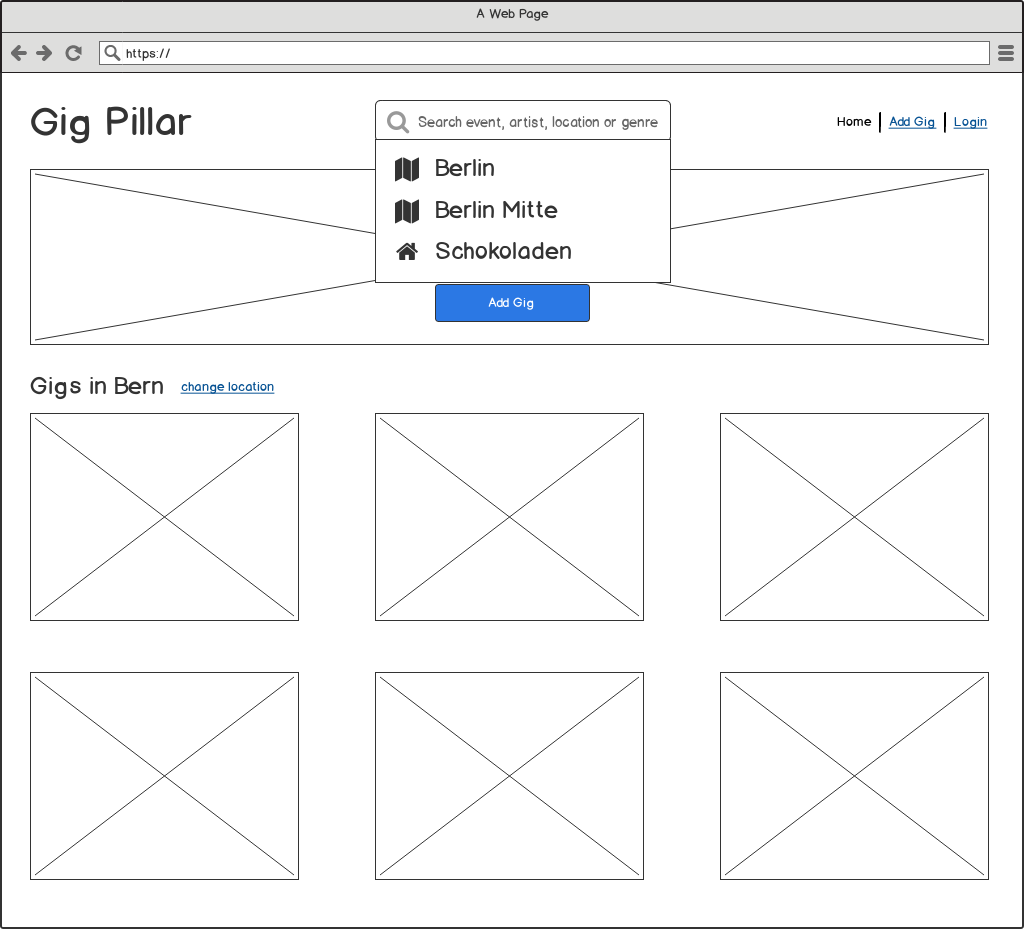
\includegraphics[width=0.95\textwidth]{mockups/homepage.png}
  \caption{Mockup: Homepage}
\end{figure}

\clearpage
\subsubsection{Suchresultate}

\begin{figure}[!htb]
  \centering
  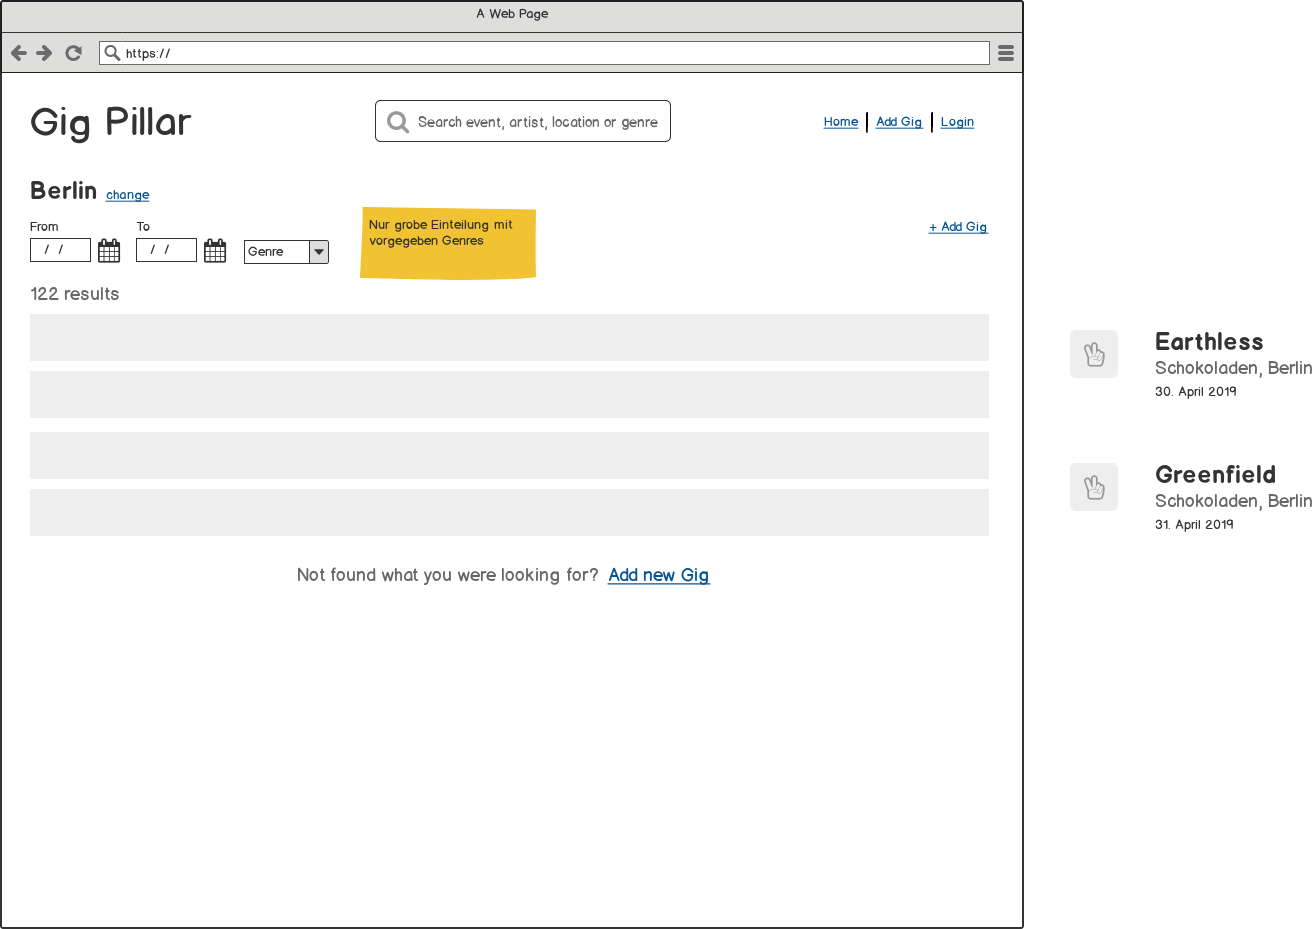
\includegraphics[width=0.95\textwidth]{mockups/search-result.png}
  \caption{Mockup: Suchresultate}
\end{figure}

\clearpage
\subsubsection{Gig Ansicht}

\begin{figure}[!htb]
  \centering
  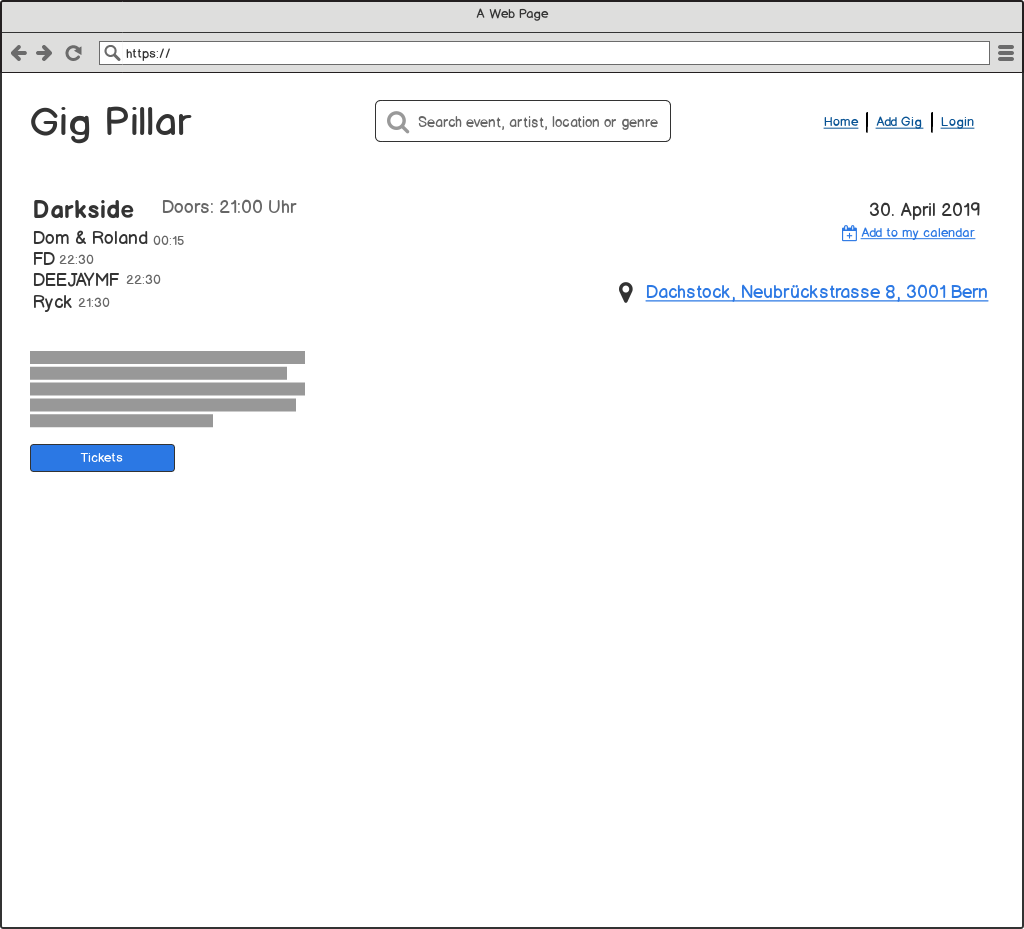
\includegraphics[width=0.95\textwidth]{mockups/event.png}
  \caption{Mockup: Gig Ansicht}
\end{figure}

\clearpage
\subsubsection{Gig erfassen}

\begin{figure}[!htb]
  \centering
  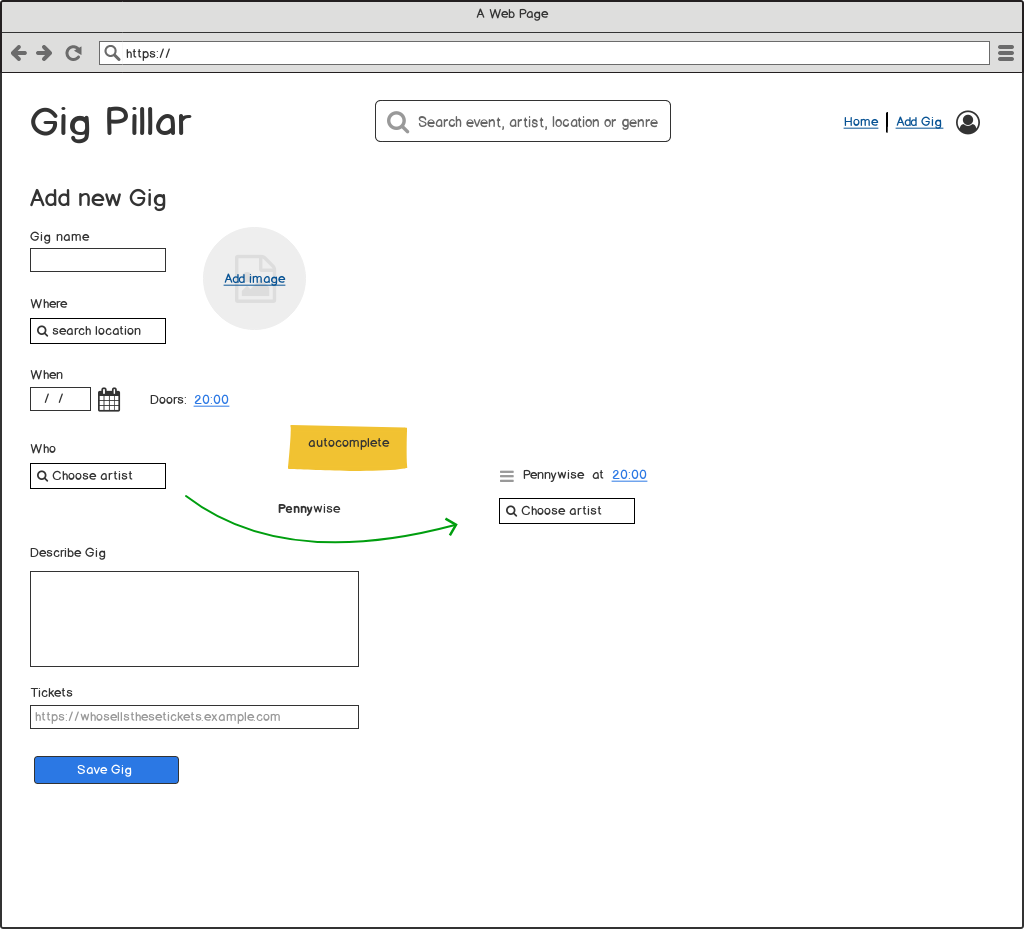
\includegraphics[width=0.95\textwidth]{mockups/add-gig.png}
  \caption{Mockup: Gig erfassen}
\end{figure}

\clearpage
\subsubsection{Benutzerprofil}

\begin{figure}[!htb]
  \centering
  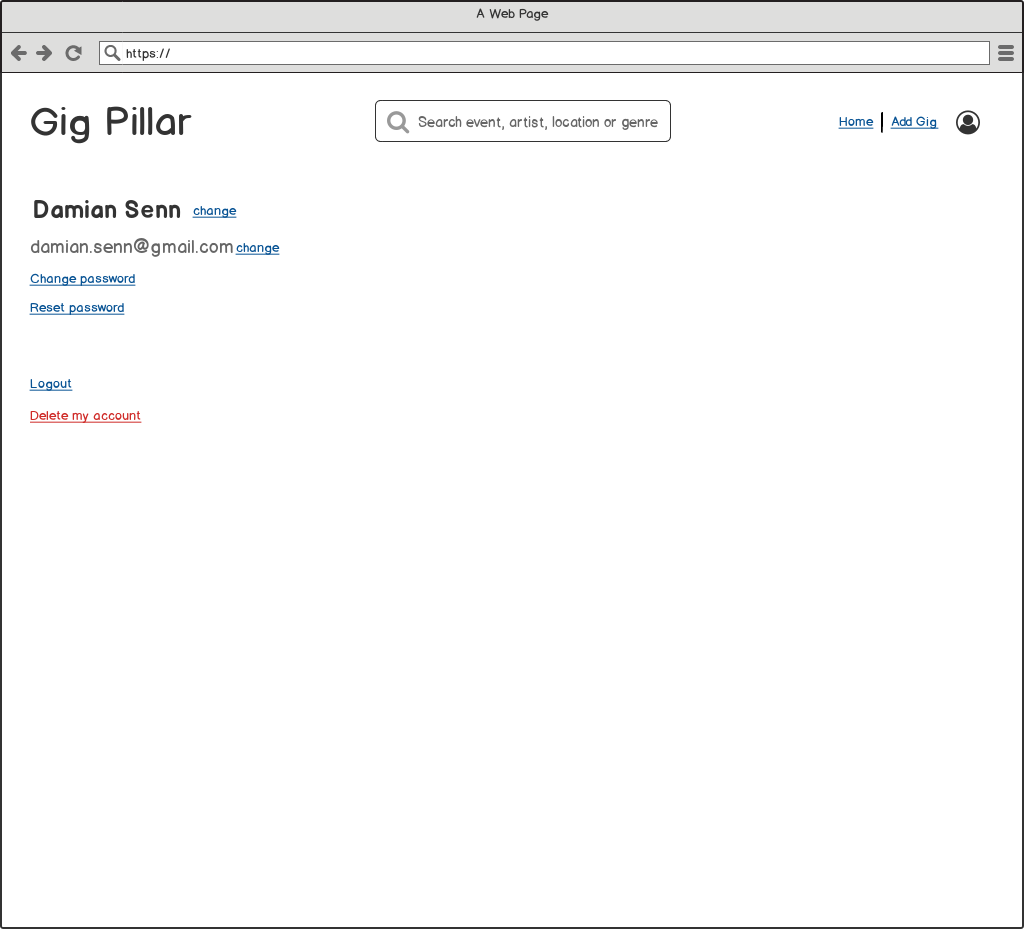
\includegraphics[width=0.95\textwidth]{mockups/profile.png}
  \caption{Mockup: Benutzerprofil}
\end{figure}

\clearpage
\section{Softwarekonzept}\label{softwarekonzept}

\subsection{Datenbankstruktur}\label{datenbankstruktur}

\begin{figure}[!htb]
  \centering
  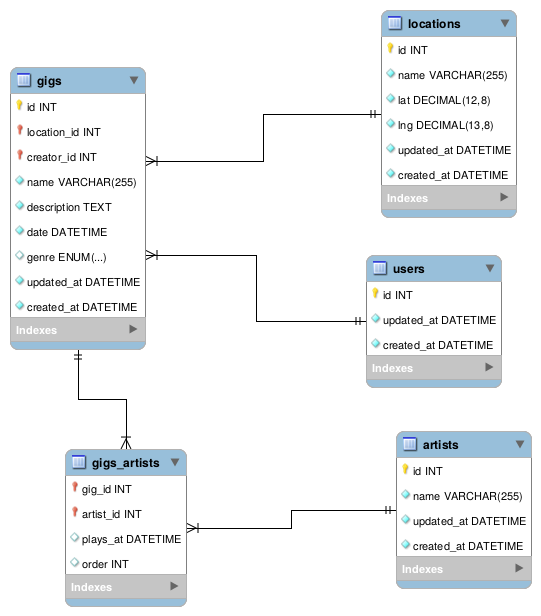
\includegraphics[width=0.95\textwidth]{konzept/erd.png}
  \caption{Entity Relationship Diagram}
\end{figure}

\section{Testkonzept}\label{testkonzept}
